\documentclass[border=3pt]{standalone}
\usepackage{tikz}
\usetikzlibrary{arrows.meta,calc}
\tikzset{pin/.style={-{Stealth[length=5pt]}}}
\begin{document}
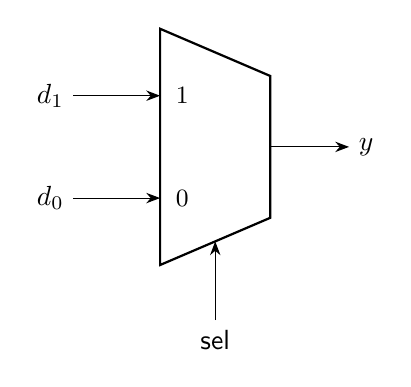
\begin{tikzpicture}[font=\sffamily]
  % trapezoid (wide left, narrow right)
  \coordinate (TL) at (0,1.5);
  \coordinate (BL) at (0,-1.5);
  \coordinate (TR) at (1.4,0.9);
  \coordinate (BR) at (1.4,-0.9);
  \draw[thick] (TL) -- (TR) -- (BR) -- (BL) -- cycle;
  % inputs
  \draw[pin] ($(BL)+(0,0.85)$)++(-1.1,0) node[left]{$d_0$} -- ($(BL)+(0,0.85)$);
  \draw[pin] ($(TL)+(0,-0.85)$)++(-1.1,0) node[left]{$d_1$} -- ($(TL)+(0,-0.85)$);
  \node[font=\small] at ($(BL)+(0.28,0.85)$) {0};
  \node[font=\small] at ($(TL)+(0.28,-0.85)$) {1};
  % output
  \draw[pin] ($(TR)!0.5!(BR)$) -- ++(1.0,0) node[right]{$y$};
  % select
  \draw[pin] ($(BL)!0.5!(BR)+(0,-1.0)$) node[below]{sel} -- ($(BL)!0.5!(BR)$);
\end{tikzpicture}
\end{document}
